\documentclass[10.5pt,a4paper]{article}
\usepackage[a4paper,left=2.6cm,right=2.6cm,top=2.6cm,bottom=2.5cm]{geometry}
\usepackage{fontspec}
\usepackage{xeCJK}
\setCJKmainfont{AR PL SungtiL GB}[AutoFakeBold=2.5]
\setCJKsansfont{AR PL SungtiL GB}[AutoFakeBold=2.5]
\usepackage{xcolor,graphicx,booktabs,array,amsmath,titlesec,enumitem,caption,float,indentfirst}
\titleformat{\section}{\bfseries\large}{\thesection}{.7em}{}
\titleformat{\subsection}{\bfseries\normalsize}{\thesubsection}{.6em}{}
\titlespacing*{\section}{0pt}{1.4em}{.6em}\titlespacing*{\subsection}{0pt}{1em}{.4em}
\pagestyle{plain}
\renewcommand{\figurename}{图}\renewcommand{\tablename}{表}
\captionsetup{font=small,labelfont=bf,labelsep=quad,skip=4pt}
\setlist[itemize]{leftmargin=1.6em,itemsep=1pt,topsep=2pt,parsep=0pt}
\setlist[enumerate]{leftmargin=1.8em,itemsep=1pt,topsep=2pt,parsep=0pt}
\setlength{\parindent}{2em}\setlength{\parskip}{0pt}\linespread{1.25}
\renewcommand{\arraystretch}{1.15}
\newcommand{\bv}[1]{\textbf{#1}}
\begin{document}

\begin{center}{\LARGE\bfseries 稀疏观测间隔下基于扩散先验的循环数据同化\\\large ——Rayleigh--B\'enard 对流，观测间隔 $K=20$\par}\end{center}

\section{研究目的}
数值求解器的预报总含有误差，数据同化用稀疏、带噪声的观测去修正它。本实验考察一种同化方法：用无条件训练的扩散模型作为状态的先验，把求解器的预报（背景场）和观测都作为引导项，通过扩散后验采样（Diffusion Posterior Sampling，DPS）得到分析场，并逐帧循环。该方法记为\textbf{扩散同化 (DPS)}。以集合卡尔曼滤波（EnKF）作为对照，纯预报（不再同化）作为参照。

本文只在\textbf{观测间隔 $K=20$}（每 20 帧同化一次，观测很稀疏）下回答两个问题：
\begin{enumerate}
\item 预报模型存在误差时，扩散同化相对 EnKF 能多降低多少未观测点误差？
\item 这一比较是否依赖 EnKF 初始集合的构造方式？
\end{enumerate}

\section{数据设置和处理}
\subsection{数据来源与划分}
数据由 Dedalus 求解二维 Rayleigh--B\'enard 对流方程生成。Rayleigh 数（Ra，描述浮力驱动的对流强度；数值越大对流越剧烈）取 $10^5$，Prandtl 数取 1。计算域 $3\times1$，水平方向周期，竖直方向 Chebyshev 配点、上下壁面无滑移，网格 $72\times24$。状态有三个通道：浮力 $b$、水平速度 $u_x$、竖直速度 $u_z$，其标准差分别为 0.256、0.164、0.158。每个轨迹由随机初始场演化得到，保存 100 帧，相邻帧相隔 35 个时间步。

\begin{table}[H]\centering\small\caption{数据集划分与用途。}
\begin{tabular}{lccp{7.2cm}}\toprule
子集 & 轨迹数 & 帧数/轨迹 & 用途\\\midrule
训练集 & 160 & 100 & 训练扩散先验；训练集快照也用于构造一种 EnKF 初始集合\\
验证集 & 20 & 100 & 选取扩散同化的引导参数与 EnKF 的膨胀系数\\
测试集 & 20 & 100 & 仅用于最终评价\\\bottomrule
\end{tabular}\end{table}

\subsection{孪生实验的构造}
以测试轨迹的帧为``真值''。观测取自真值：随机选 1\%（17 / 1728）格点，三个通道同时观测，叠加标准差 0.1 的高斯噪声（约为 $b$、$u$ 通道标准差的 40\%--60\%）；观测位置和噪声由随机种子决定，三种方法在同一轨迹、同一种子下使用完全相同的观测。模型误差由预报求解器的参数失配制造：求解器取 Ra$=5\times10^4$，而真值为 $10^5$。预处理上，数据按通道标准化后进入扩散先验；评价在物理量纲下进行。

\section{实验方法}
\subsection{扩散同化 (DPS)}
\textbf{先验。}U-Net（基础通道数 16）在训练集的帧上按标准扩散目标无条件训练 200 个 epoch；训练中不使用观测与背景场，同化时不再训练。

\textbf{后验采样。}采样自纯噪声开始（100 步，起始时刻 $t=0.4$），每步在先验得分上叠加三类引导：
(1) 观测项，仅在观测点上计算，权重由 $\sigma_{\rm obs}=0.05$ 决定；
(2) 背景项，在全场计算，约束分析场接近求解器预报，权重由 $\sigma_{\rm bg}=0.3$ 决定；
(3) 散度惩罚，系数 0.3。
每个窗口取 32 个样本，对每个样本做无散度、无滑移投影后取均值作为分析场。$\sigma_{\rm obs}$ 是引导强度，不等同于观测噪声标准差。

\textbf{循环。}同化时刻：用求解器把上一次分析场预报到当前帧作为背景，再采样得到分析场；非同化时刻：直接取求解器预报。第一次同化没有背景，只使用观测。
\begin{figure}[H]\centering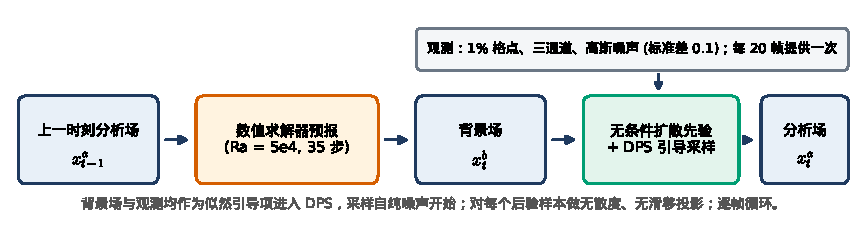
\includegraphics[width=\linewidth]{report_fig_k20/workflow.pdf}\caption{扩散同化的循环流程。}\end{figure}

\subsection{对照方法}
\textbf{EnKF}：20 个成员的随机 EnKF，每个成员的观测叠加独立噪声，观测误差标准差 0.1，乘性膨胀，不使用局地化；预报模型与扩散同化相同（Ra$=5\times10^4$）。\textbf{纯预报}：只在起始同化时刻用观测得到分析场，此后仅由求解器预报，不再同化。

\section{实验设置}
\subsection{误差来源}
\begin{table}[H]\centering\small\caption{本实验中的误差来源。}
\begin{tabular}{p{2.2cm}p{9.2cm}}\toprule
误差来源 & 设定\\\midrule
观测噪声 & 零均值高斯，标准差 0.1，三个通道相同\\
观测稀疏性 & 1\% 格点；每 20 帧提供一次（$K=20$）\\
模型误差 & 求解器 Ra$=5\times10^4$，真值 Ra$=10^5$\\\bottomrule
\end{tabular}\end{table}

\subsection{EnKF 的三种初始集合}
EnKF 必须有 20 个初始成员，构造方式影响结果，本文比较三种，它们使用的信息不同。
\begin{table}[H]\centering\small\caption{三种 EnKF 初始集合与对应的同化起止。}
\begin{tabular}{clp{5.6cm}p{3.1cm}}\toprule
编号 & 名称 & 构造方式 & 是否含真值信息\\\midrule
I & 中心加扰动 & 以扩散同化第 0 帧的分析场为中心，加去均值的物理一致扰动（幅度 0.1 倍参考标准差）；从第 0 帧起同化 & 否，但中心借用了扩散同化的结果\\
II & 训练集快照 & 取 20 个训练轨迹的各一帧作为成员；从第 0 帧起同化 & 否\\
III & 滞后积分 (lag) & 取\textbf{同一测试轨迹}真值的第 0--19 帧，各自用求解器积分到第 40 帧作为成员；从第 40 帧起同化 & \textbf{是}（前 20 帧真值）\\\bottomrule
\end{tabular}\end{table}
设置 I、II 中三种方法都从第 0 帧开始连续同化，两个设置里的扩散同化与纯预报是\\textbf{同一次运行}（只有 EnKF 的初始集合不同），所以表中这两列数值相同；设置 III 中扩散同化与纯预报在第 40 帧\textbf{冷启动}（该帧只用观测，没有历史），EnKF 带着滞后积分得到的集合开始。

\subsection{评价与调参}
指标为\textbf{未观测点 RMSE}：在没有观测的格点上，三个通道合并计算分析场（非同化帧为预报场）与真值的均方根误差，物理量纲。所有设置统一在第 40--99 帧（共 60 帧）上取平均，$K=20$ 时该窗口内同化发生在第 40、60、80 帧。随机种子取 42、43、44，每个种子 20 个测试轨迹。扩散同化的引导参数沿用前期在验证集上（$K=1$）选定的值，未针对 $K=20$ 重调；EnKF 的膨胀系数在验证集上选：设置 I、II 取 1.4，设置 III 取 2.0（扫描区间 1.0--2.0 的上边界）。配对差为各轨迹（对三个种子取均值）上 EnKF 与扩散同化的 RMSE 之差，区间为 20 个轨迹上的 95\% $t$ 置信区间。

\section{实验结果和分析}
\subsection{$K=20$ 主对比}
\begin{table}[H]\centering\small\caption{$K=20$，第 40--99 帧未观测点 RMSE。括号内为 3 个种子的最小与最大值。``配对差''为 EnKF 减扩散同化的 RMSE（正值表示扩散同化更优）；``更优轨迹数''为 20 个轨迹中扩散同化更优的个数。}
\resizebox{\linewidth}{!}{\begin{tabular}{clccccc}\toprule
编号 & EnKF 初始化 & 扩散同化 (DPS) & EnKF & 纯预报 & 配对差（95\% 区间） & 更优轨迹数\\\midrule
I & 中心加扰动 & 0.0361（0.0356--0.0363） & 0.0408（0.0401--0.0420） & 0.0510（0.0489--0.0530） & $+0.0047\pm0.0012$ & 19/20 \\
II & 训练集快照 & 0.0361（0.0356--0.0363） & 0.0362（0.0343--0.0384） & 0.0510（0.0489--0.0530） & $+0.0002\pm0.0019$ & 10/20 \\
III & 滞后积分 (lag) & 0.0356（0.0329--0.0392） & 0.0292（0.0288--0.0295） & 0.0412（0.0375--0.0454） & $-0.0065\pm0.0016$ & 0/20 \\
\bottomrule\end{tabular}}\end{table}
\begin{figure}[H]\centering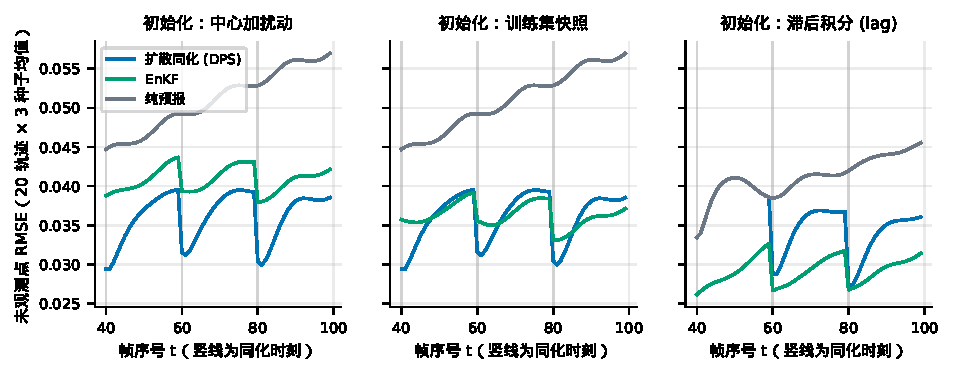
\includegraphics[width=\linewidth]{report_fig_k20/curves.pdf}\caption{不同 EnKF 初始化下三种方法的逐帧误差。}\end{figure}
\begin{figure}[H]\centering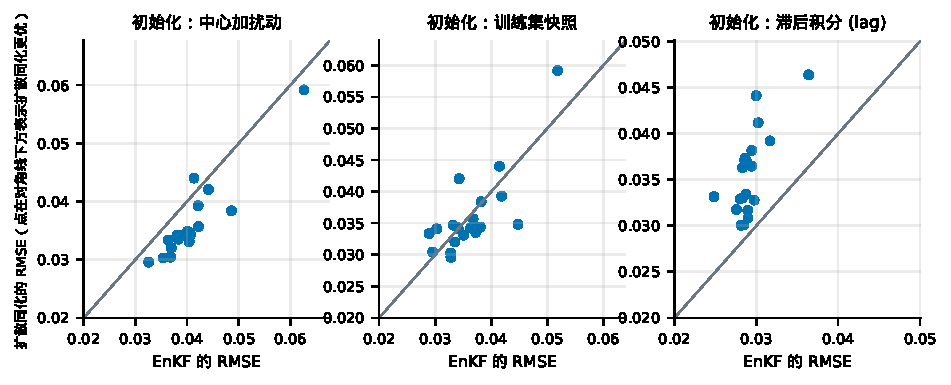
\includegraphics[width=\linewidth]{report_fig_k20/scatter.pdf}\caption{逐轨迹配对比较（3 个种子取均值）。}\end{figure}

纯预报的未观测点 RMSE 为 0.0510（设置 I、II）与 0.0412（设置 III；起点不同，误差随预报时间增长，故两者不可直接比较），扩散同化与 EnKF 在各设置下都低于纯预报，说明 $K=20$ 时同化仍然有效。三种 EnKF 初始化下两种方法的相对关系并不一致：设置 I 中扩散同化比 EnKF 低 12\%，配对差 0.0047$\pm$0.0012（区间不含 0），19/20 个轨迹更优；设置 II 中两者持平（0.0361 对 0.0362），配对差 0.0002$\pm$0.0019（区间含 0），10/20 个轨迹更优；设置 III 中 EnKF 更优，扩散同化的 RMSE 高 22\%，配对差 -0.0065$\pm$0.0016，仅 0/20 个轨迹更优。

\subsection{EnKF 初始化的影响}
\begin{figure}[H]\centering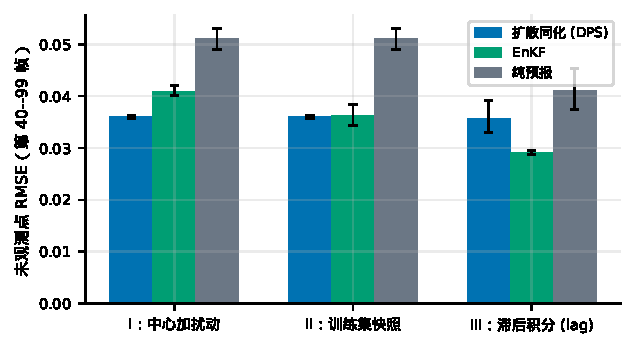
\includegraphics[width=.72\linewidth]{report_fig_k20/bar.pdf}\caption{三种 EnKF 初始化下的未观测点 RMSE（须为 3 个种子的范围）。}\end{figure}
设置 I 的 EnKF 以扩散同化的第 0 帧分析场为中心，借用了扩散同化的结果；设置 II 的集合只来自训练集，与扩散同化的先验信息来源对等，是三者中最不含额外信息的对照；设置 III 的集合含有测试轨迹真值的前 20 帧。因此，$K=20$ 下扩散同化与 EnKF 的相对优劣\textbf{取决于 EnKF 如何初始化}：在信息来源对等的设置 II 中二者无显著差别，在借用了扩散同化结果的设置 I 中扩散同化略优，在含真值信息的设置 III 中 EnKF 更优。设置 III 还有两点不对等：EnKF 带有历史信息，而扩散同化在第 40 帧冷启动、没有历史；该集合在第 40 帧的离散度（约 0.004）远小于实际误差（约 0.030），需要较大的膨胀系数（2.0）补偿。

\subsection{小结与局限}
在本实验设置下（预报 Ra 失配、1\% 观测、噪声 0.1、$K=20$），可以得到的结论有三条。(1) 同化相对纯预报有改善，这一点在三种初始化下都成立。(2) 当 EnKF 的初始集合只来自训练集时（设置 II），扩散同化与调优的 EnKF 无显著差别（配对差 0.0002$\pm$0.0019）。本实验\textbf{不能}支持``长间隔观测下扩散同化优于 EnKF''。(3) 当 EnKF 的集合含真值信息时（设置 III），EnKF 更优；这一差距有多少来自真值信息、有多少来自方法本身，本实验没有对照，不能判断。\par 主要局限：扩散同化的引导参数只在 $K=1$ 下选定，未针对 $K=20$ 调优；设置 III 的 EnKF 膨胀系数处于扫描边界；设置 II 的膨胀系数沿用设置 I 的验证结果；评价窗口仅 60 帧，该窗口内只有 3 次同化；只有一档模型误差（Ra 失配）；种子数为 3。下一步应在 $K=20$ 下为扩散同化重新调参，并补做一个既不含真值、也不借用扩散同化结果的 EnKF 初始化（例如独立预热的集合）。
\end{document}
